\documentclass[10pt]{article}
\usepackage[cp1251]{inputenc}
\usepackage[english]{babel}
\usepackage{url}
\usepackage{graphicx,DCCN2015_en}



\makeatletter
\c@page=1 % Number will be set by publisher.
          
\makeatother


% Proper title, should be and will be capitalized
\title{Low-priority Queue Fluctuations in Tandem of Queuing Systems under Cyclic Control with Prolongations}
\author{V.~M.~Kocheganov$^1$, A.~V.~Zorine$^1$}
\company{$^1$ Departament of Applied Probability Theory, N.~I.~Lobachevsky State University of Nizhny Novgorod, Nizhny Novgorod, Russia}
\email{kocheganov@gmail.com, zoav1602@gmail.com}


%%%%%%%%%%%%%%%%%%%%%%%%%%%%%%%%

\begin{document}

\maketitle

%%%%%%%%%%%%%%%%%%%%%%%%%%%%%%%%%%%%%%%%%%%%%%%%%%%%%%%%%%%%%%
\begin{abstract}
A tandem of queuing systems is considered. Each system has a high-priority input flow and a low-priority input flow which are conflicting. In the first system, the customers are serviced in the class of cyclic algorithms. The serviced high-priority customers are transferred from the first system to the second one  with random delays and become the high-priority input flow of the second system. In the second system, customers are serviced in the class of cyclic algorithms with prolongations. Low-priority customers are serviced when their number exceeds a threshold. A mathematical model is constructed in form of a multidimensional denumerable discrete-time Markov chain. The recurrent relations for partial probability generating functions for the low-priority queue in the second system are found.

\keywords{tandem of controlling queuing systems, cyclic algorithm with prolongations, conflict flows, multidimensional denumerable discrete-time Markov chain}
\end{abstract}
%%%%%%%%%%%%%%%%%%%%%%%%%%%%%%%%%%%%%%%%%%%%%%%%%%%%%%%%%%%%%%


\section{Introduction}
Conflict traffic flows control at a crossroad is one of the classical problem of queuing theory. The problem has been solved for different classes of algorithms: the class of algorithms with a cyclic fixed rhythm, with renewals ("with a loop") with dynamic priorities, etc. However, several (two in our case) consecutive crossroads are of great interest, because in a real life after car passed one highway intersection it finds itself at another one. In other words, output flow of the first intersection forms input flow of the second intersection. Hence, the second input flow no longer has simple probabilistic structure known a priori (for example, non-ordinary Poison process) and knowledge about service algorithm should be taken into account to deduce formation properties of the first output flow.

In [1] the problem of tandem of two crossroads was carried out and rigorous probabilistic model was built. At each of the intersections, in addition to the high priority flow, there was the traffic flow "in the perpendicular direction", with lower priority. The service of the flows on first intersection is supposed to be in the class of cyclic algorithms and in the of cyclic algorithms with prolongations on the second intersection. Over and above, vehicles could not turn from one conflict direction to another. In this paper we continue the study of described problem and deepen in low priority flow of the second intersection investigation.
\subsection{Subsection heading here}

Subsection text here. Maximum level of depth allowed for defining sections is 2.



\section{Submitted paper}

The full source text using \TeX{} as well as all auxiliary
materials, namely,
\begin{itemize}
  \item .tex file,
  \item pictures in .pdf (or .eps) format (if available),
  \item the paper in pdf format
\end{itemize}
have to be submitted as a zip-archive.

The name of the archive should be
\textbf{Surname1\_Surname2\_Surname3.zip}.

\section{Font}

Type the text of the paper in 10 points, regular. Each
paragraph is to be indented 5~mm, and their intervals must be 0
points before and after.

\section{Mathematical formulae and references}

To make references to mathematical expressions, it is
recommended to use \LaTeX{} mechanism. For example, the formula
given below
\begin{equation}
\label{eq:1}
P(n,t)=\frac{\partial^n B(t)}{\partial t^n}
\end{equation}
can be referred as \eqref{eq:1}.

\section{Theorems and proofs}

Theorems are defined like follows
\begin{thm}\label{thm1}
Text of the theorem.
\end{thm}

\begin{proof}
Proof of Theorem \ref{thm1}. If using such reference, you need
to recompile your paper with \LaTeX{} twice.
\end{proof}


\section{Figures and tables}

Figures should be provided in PDF or EPS format. Raster pictures have
to be made with maximal resolution (minimal 300 dots per inch).

\begin{figure}[h!]
   \centering
    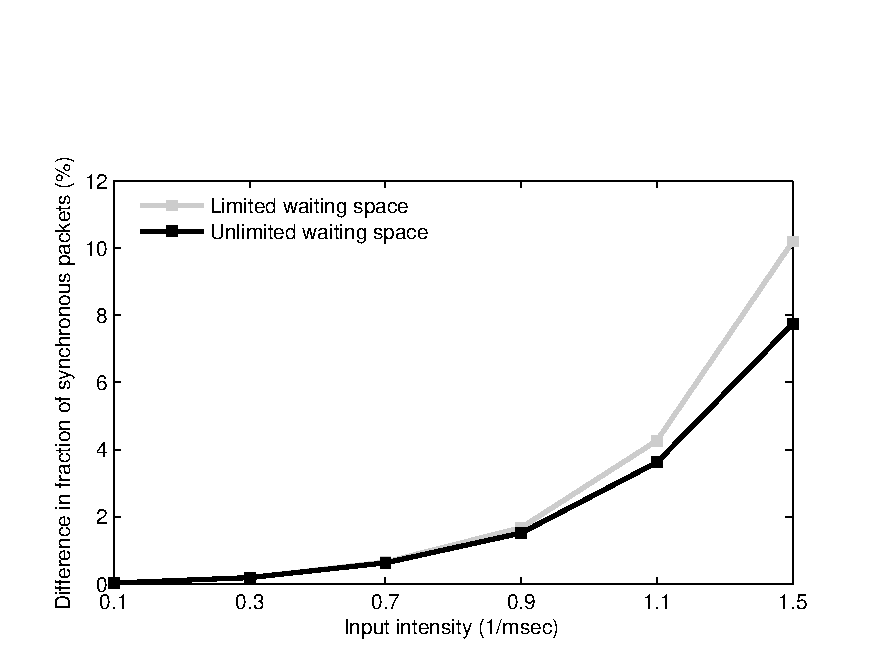
\includegraphics[width=\textwidth]{1.pdf} % or {1.eps} in case of EPS format of the picture
    \caption {Difference in fractions of synchronous packets for $W=16$.}
    \label{pic1}
\end{figure}

\begin{table}[h!]\begin{center}
\label{tab}
\begin{tabular}{|c||c|c|c||c||c|c|c|}\hline
  Parameter & T & E & $\Delta$, \% & Parameter & T & E & $\Delta$, \% \\ \hline \hline
  $\rho_{1}^{(1)}$ & 0,187 & 0,194 & 3,7 &  $\rho_{1}^{(2)}$ & 0,127 & 0,120 & 5,6 \\ \hline
  $\rho_{2}^{(1)}$ & 0,073 & 0,072 & 1,4 &  $\rho_{2}^{(2)}$ & 0,052 & 0,053 & 1,9 \\ \hline
  $\rho_{3}^{(1)}$ & 0,148 & 0,147 & 0,7 &  $\rho_{3}^{(2)}$ & 0,103 & 0,103 & 0,0 \\ \hline
  $\rho_{4}^{(1)}$ & 0,036 & 0,036 & 0,0 &  $\rho_{4}^{(2)}$ & 0,026 & 0,027 & 3,7 \\ \hline \hline
  $C^{(1)}$ & 0,479 & 0,476 & 0,6 & $C^{(2)}$ & 0,656 & 0,640 & 2,5 \\ \hline \hline
  $C_{1}^{*}$ & 0,341 & 0,339 & 0,6 & $C_{3}^{*}$ & 0,323 & 0,329 & 1,8 \\ \hline
  $C_{2}^{*}$ & 0,296 & 0,298 & 0,7 & $C_{4}^{*}$ & 0,286 & 0,286 & 0,0 \\ \hline
\end{tabular}\caption{Comparison of system parameters.}
\end{center}\end{table}

The figures and tables must be numbered, have a self-contained
caption and referred in the main text. Figure and table
captions are placed below the object and centered. Also, avoid
placing figures and tables before their first mention in the
text. Use the abbreviation "Fig." even at the beginning of a
sentence.

The authors are recommended not to use characters smaller than
9 point in figures. Do not use abbreviations in the titles
unless they are unavoidable.


\section{Conclusion}

Place a full list of references \cite{Bianchi00, VL02, neuts, GPSS, url} at the end of the paper. List
the references according to the order of their appearance in
the text.

%{\bf Acknowledgments.}

\begin{thebibliography}{99}
\bibitem{Bianchi00}  %% citation code
Bianchi G. Performance Analysis of the IEEE 802.11 Distributed
Coordination Function ~// IEEE Journal on Selected Areas in
Communications. 2000. V. 18. P.~535-547.

\bibitem{VL02} Vishnevsky V.~M., Lyakhov A.~I. IEEE 802.11
    Wireless LAN: Saturation Throughput Analysis with Seizing
    Effect Consideration
// Cluster Computing. 2002. V. 5. P. 133-144.

\bibitem{neuts} Neuts M.~F.  Structured Stochastic
    Matrices of M/G/1 Type and Their Applications. Marcel
    Dekker, New York, 1989.

\bibitem{GPSS} Schriber T.~J. Simulation using GPSS. John
    Wiley \& Sons, 1974.
    
\bibitem{url} National Center for Biotechnology Information, \url{http://www.ncbi.nlm.nih.gov}

\end{thebibliography}

\end{document}
